\documentclass[a4paper]{article}
\usepackage[margin=0.5cm]{geometry} % 设置极窄边距(5mm)以容纳大网格
\usepackage{tikz}

\begin{document}

% 移除页眉页脚和页码,保证纯净的网格
\pagestyle{empty}
\centering

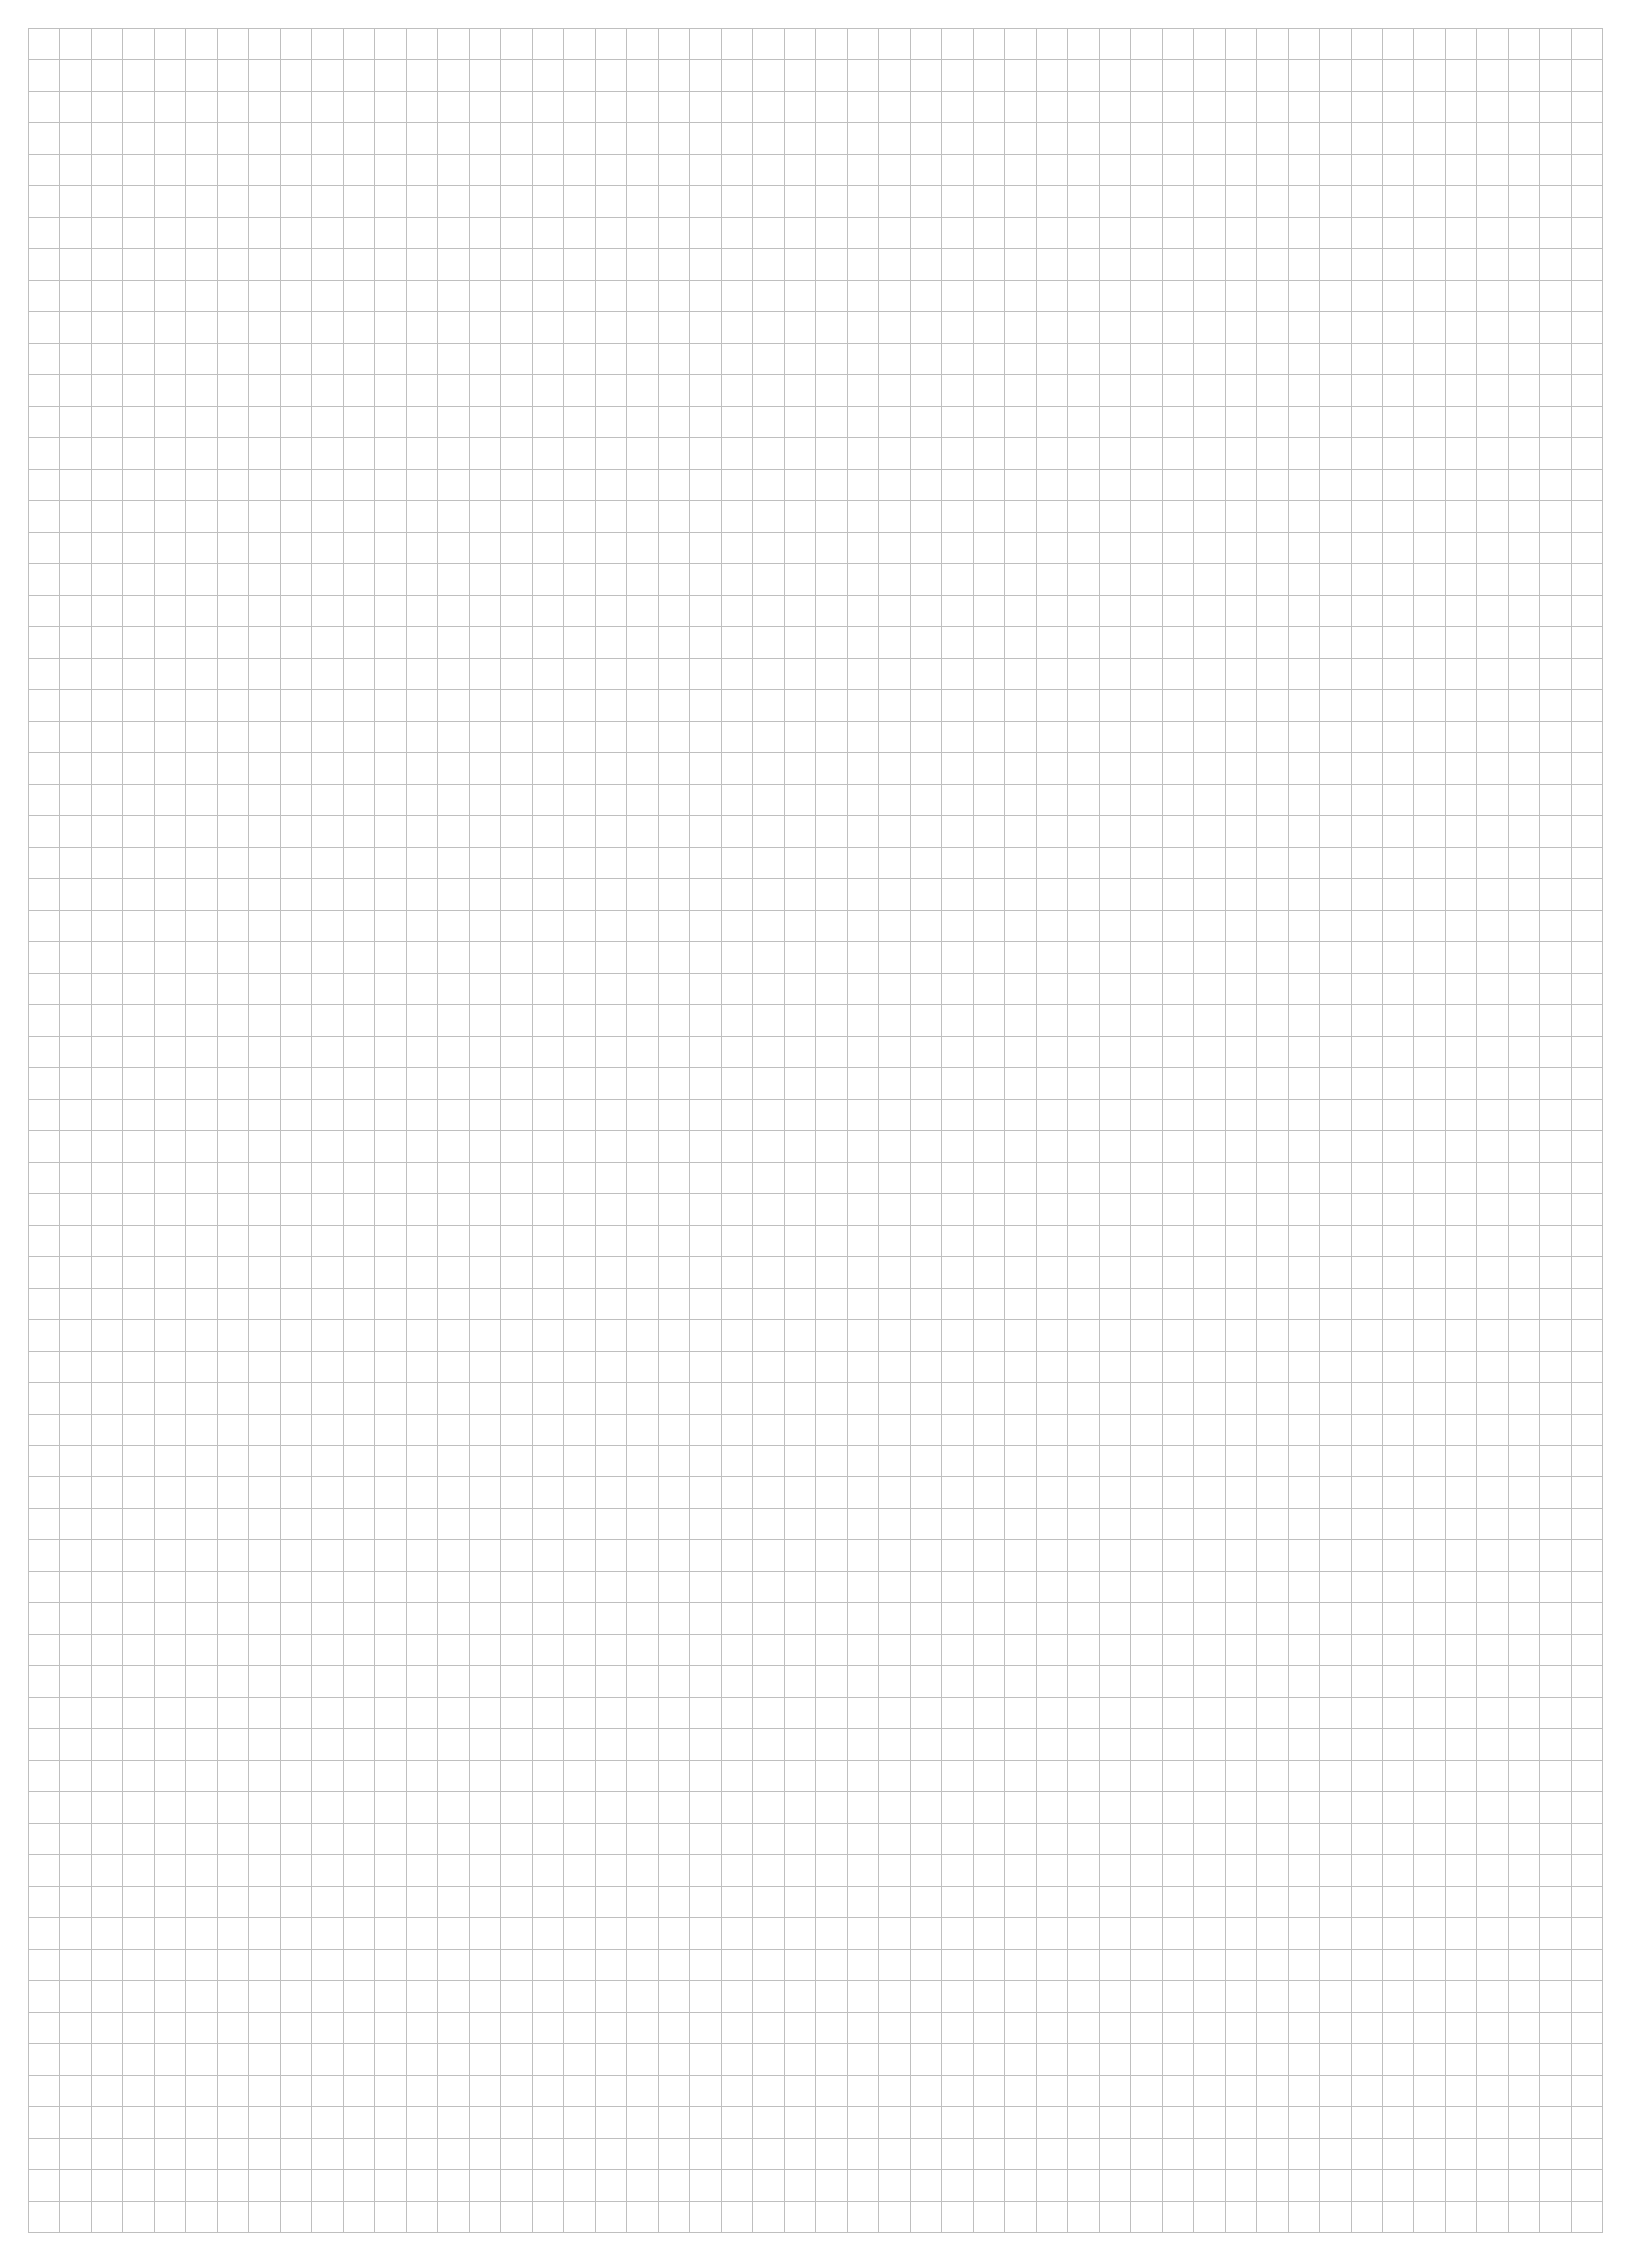
\begin{tikzpicture}
    % 定义参数
    % step=0.4cm: 格子边长 4mm
    % (0,0) grid (20,28):
    %   宽度 = 50格 * 0.4cm = 20cm
    %   高度 = 70格 * 0.4cm = 28cm
    % gray!50: 使用50%灰度,避免线条太黑抢眼
    % very thin: 使用极细线条

    \draw[step=0.4cm, gray!50, very thin] (0,0) grid (20, 28);

    % 可选:如果你需要给外边框加粗,可以取消下面这行的注释
    % \draw[thick, black] (0,0) rectangle (20, 28);
\end{tikzpicture}

\end{document}